% !TeX program = pdflatex
% Compile: tectonic main.tex   (or pdflatex+bibtex twice)
% Submission: switch [preprint] -> [review] for anonymous *ACL submission.
\documentclass[11pt]{article}
\PassOptionsToPackage{hyphens}{url}
\usepackage[preprint]{acl}
\usepackage{times}
\usepackage[T1]{fontenc}
\usepackage[utf8]{inputenc}
\usepackage{amsmath,amssymb}
\usepackage{booktabs}
\usepackage{graphicx}
\usepackage{multirow}
\usepackage{subcaption}
\usepackage{enumitem}
\graphicspath{{figures/}}

\newcommand{\ecsadj}{\mbox{ECS\textsubscript{adj}}}
\newcommand{\aj}{\mathrm{AJ}}
\newcommand{\holm}[1]{$p_{\mathrm{Holm}}{=}#1$}

\title{Do LLM Self-Explanations Tell One Story?\\A Chance-, Ceiling-, and Reliability-Corrected Audit of Cross-Paradigm Agreement}

% TODO(authors): fill affiliations + emails before submission.
% Note: academic titles (Dr.) are conventionally omitted in *ACL author blocks.
\author{Aditya Shrivastav \\
  Affiliation \\
  \texttt{email@domain} \And
  Aditya Kumar \\
  Affiliation \\
  \texttt{email@domain} \And
  Swathi Jagdale \\
  Affiliation \\
  \texttt{email@domain}}

\begin{document}
\maketitle

\begin{abstract}
Large language models are routinely asked to explain their own predictions through interchangeable-looking devices: token highlighting, free-text rationales, counterfactual rewrites, and importance rankings. We ask whether these elicitation paradigms actually name the same evidence, in a pre-registered study of 3 model families (two open-weight, one proprietary) $\times$ 4 datasets (2{,}400 instances), including the shortcut-resistant CAD-IMDb. Because raw token overlap is confounded by chance and by set-size geometry, we introduce \ecsadj{}: an exact-hypergeometric chance correction combined with a geometric ceiling correction and paradigm-balanced aggregation; and because the elicitation instruments are themselves unreliable, we measure per-strategy self-consistency ceilings under three independent prompt rewordings and apply classical reliability disattenuation. Agreement exceeds chance in every model$\times$dataset cell (12/12, Holm $p{\le}0.0012$; pooled \ecsadj{} $=0.43$ on a 0=chance, 1=ceiling scale), but is far from uniform: after reliability correction, extraction$\leftrightarrow$counterfactual divergence largely disappears (corrected agreement $0.88$--$0.94$), whereas rationale-involving divergence persists (rationale--counterfactual $0.39$, 95\% CI $[0.35,0.43]$). Two models explaining the same input with the same paradigm agree more than one model explaining it with two paradigms, on all four datasets. Consensus tokens are causally load-bearing---erasing them flips predictions $2.0$--$2.7\times$ more than matched random controls---yet a pre-registered test finds agreement does \emph{not} predict simulatability under explanation-independent perturbations. Explanation paradigms are not interchangeable views of one underlying story, and internal agreement cannot be assumed to certify downstream utility.
\end{abstract}

\section{Introduction}
\label{sec:intro}

When practitioners want to know \emph{why} an LLM made a prediction, they ask it---and the asking can take several standard forms: score the importance of each token \citep{huang2023can}, give a one-sentence rationale \citep{camburu2018esnli,wiegreffe2021measuring}, produce a minimal edit that would flip the label \citep{ross2021explaining}, or rank the most important words. These paradigms are used interchangeably in practice, as if they were different renderings of one underlying explanation. For post-hoc explainers of classical models, the ``disagreement problem'' \citep{krishna2022disagreement} showed that different attribution methods routinely name different evidence. Whether the same fragmentation afflicts the \emph{self}-explanations of instruction-tuned LLMs---one model, one prediction, four ways of asking---is the question of this paper.

Answering it is mostly a measurement problem, with three obstacles. First, \emph{chance}: two random token subsets of a short input overlap substantially, so raw Jaccard rewards brevity. Second, \emph{geometry}: a counterfactual edit touches 1--2 tokens while a salience list contains 3--10, capping achievable Jaccard far below~1 for some pairs but not others, so a flat average measures set-size geometry more than agreement. Third, \emph{reliability}: the instruments are themselves noisy---under mild prompt paraphrase, per-strategy self-agreement ranges from $0.62$ to $0.90$---so a low observed value is ambiguous between \emph{real paradigm divergence} and \emph{unreliable elicitation}.

We address all three. Our estimator, \ecsadj{}, normalizes each pairwise Jaccard by its exact hypergeometric expectation (chance floor) and its size-determined maximum (ceiling), then aggregates the five cross-paradigm pairs into three paradigm-level contrasts with equal weight. Per-strategy test--retest reliabilities, measured with a paraphrase ablation on every model, feed a classical Spearman disattenuation \citep{spearman1904proof}: if the instruments were perfectly reliable, how much would the paradigms agree? All estimands, test families, exclusion floors, and amendments were pre-registered before collection---including a fourth, counterfactually-revised dataset \citep{kaushik2020learning} that blunts the ``near-solved benchmark'' objection, and a simulatability bridge \citep{chen2024models} whose result we report as the null it produced.

\paragraph{Findings.} On 2{,}400 instances (3 models $\times$ 4 datasets $\times$ 200), elicited at temperature 0 through frozen, literature-anchored prompts:
\begin{enumerate}[leftmargin=*,itemsep=1pt,topsep=2pt]
\item \textbf{Above-chance agreement everywhere.} Complete-case \ecsadj{} is positive in all 12 model$\times$dataset cells (range $0.28$--$0.62$; Holm-corrected sign-flip $p\le0.0012$ in every cell), pooled $0.43$---roughly $40\%$ of the way from chance to the geometric ceiling (\S\ref{sec:above-chance}).
\item \textbf{Agreement is structured by paradigm distance, and reliability correction sharpens the structure.} Observed agreement orders extraction--perturbation $>$ extraction--rationalization $>$ rationalization--perturbation (complete-case within-instance means $0.615 > 0.395 > 0.286$). After disattenuation, extraction$\leftrightarrow$counterfactual pairs approach the ceiling (H--CF $0.88$, RO--CF $0.96$)---their observed divergence is largely elicitation noise---while every rationale-involving pair stays far below 1 (R--CF $0.39$, CI $[0.35,0.43]$): free-text rationales genuinely select different evidence (\S\ref{sec:ladder}).
\item \textbf{Explanations are paradigm-shaped more than model-shaped.} Two \emph{different} models explaining the same input with the same strategy agree more than \emph{one} model explaining it with two strategies, on all 4 datasets (matched paired contrast, all CIs above 0; \S\ref{sec:crossmodel}).
\item \textbf{Consensus is causally load-bearing but not decision-useful.} Erasing the tokens that $\ge$3 strategies agree on flips the model's own prediction $2.0$--$2.7\times$ more often than occurrence-matched random controls (all models, both operators, \holm{0.0002}; \S\ref{sec:erasure}). Yet agreement does not predict simulatability under explanation-independent perturbations: explanations barely improve a simulator over a no-explanation baseline (pooled gains $-0.015$ to $+0.016$), and the pre-registered association between \ecsadj{} and simulatability gain is null (\S\ref{sec:simulatability}).
\end{enumerate}

We release the full pipeline: frozen prompts with hashes, curated datasets with datasheets, per-instance artifacts, seeds, and the pre-registration with dated amendments.

\section{Related Work}
\label{sec:related}

\paragraph{Faithfulness and self-consistency.}
Interpretability work distinguishes an explanation being \emph{plausible} from being \emph{faithful} to the model's computation \citep{jacovi2020towards,lyu2024towards}. \citet{turpin2023language} showed chain-of-thought can misstate the true drivers of predictions, and \citet{madsen2024selfexplanations} found self-explanation faithfulness is model- and task-dependent. \citet{parcalabescu2024measuring} argue most existing tests---including erasure-style checks---measure \emph{self-consistency} rather than faithfulness. We adopt that framing: all our axes are consistency measures, and none certifies faithfulness (\S\ref{sec:limitations}).

\paragraph{Agreement between explanation methods.}
The disagreement problem \citep{krishna2022disagreement} quantified how post-hoc attribution methods conflict for classical models; for LLMs, \citet{huang2023can} compared self-generated saliency to LIME/occlusion and \citet{randl2024evaluating} report related single-model reliability results. We differ in three ways: we compare four \emph{self}-elicitation paradigms (not model-external attributions) across three model families and four datasets; we correct for both chance and set-size ceiling with an exact null; and we read observed agreement against measured instrument reliability---to our knowledge the first application of psychometric disattenuation to explanation agreement.

\paragraph{Counterfactuals and simulatability.}
Minimal contrastive editing \citep{ross2021explaining} defines the counterfactual construct we elicit, and \citet{dehghanighobadi2025can} study LLM self-counterfactuals in isolation. \citet{mothilal2021towards} formalize why attribution (sufficiency-oriented) and counterfactual (necessity-oriented) evidence diverge by construction; our rationalization--perturbation results quantify that divergence once chance, ceiling, and reliability are controlled. Counterfactual simulatability \citep{chen2024models} operationalizes an explanation's practical value---does it help an observer predict model behavior on perturbed inputs?---and we pre-registered a bridge from agreement to a strategy-fair variant of it (\S\ref{sec:simulatability}). For verbalized confidence we replicate the overconfidence clustering of \citet{xiong2024can} and \citet{tian2023just}.

\section{Measuring Cross-Paradigm Agreement}
\label{sec:method}

\subsection{Four elicitation paradigms, one token space}
\label{sec:paradigms}

For each instance the model first classifies the text; every explanation is then elicited for the model's \emph{own} predicted label (a label-conditioned, post-hoc protocol; see \S\ref{sec:limitations} for what this implies). The four strategies are:
\textbf{H} (highlighting): score every word 1--10 for importance \citep{huang2023can}; the evidence set is a length-proportional top-$k$, with repeated words aggregated by max score and score ties broken alphabetically in the normalized token space for determinism. The rule as registered and as implemented is $k=\max(3,\,\mathrm{round}(L/5))$, where $L$ counts the input's whitespace tokens that are not pure punctuation, capped at the number of valid scored tokens. It adapts \citet{huang2023can}'s length-proportional selection with two disclosed deviations: a floor of 3 rather than 1, and rounding rather than the floor function (their §III-B prints $\min(1,\lfloor L/5\rfloor)$, which yields $k\le1$ for every input and contradicts their own top-3 prompt; the intended reading is $\max$). Because $k$ is a design choice with no canonical value, we also report a size-robust composite built from overlap coefficients rather than Jaccard---a post-hoc recombination of the plan's pre-registered overlap secondary---which preserves the paradigm ordering (E--P $0.786$ $>$ E--R $0.689$ $>$ R--P $0.526$ pooled); a fully $k$-free graded-weight variant is left to future work.
\textbf{R} (rationale): a one-sentence free-text explanation \citep{wiegreffe2021measuring}; content words are extracted with a POS filter.
\textbf{CF} (counterfactual): a minimal edit that flips the label, constrained to $\le\frac13$ of words \citep{ross2021explaining}; the evidence set is the tokens changed, and validity requires the model's verified label flip.
\textbf{RO} (rank ordering): the 5 most important words, ranked.
Three paradigms group these four strategies: \emph{extraction} (E) = \{H, RO\}, \emph{rationalization} (R) = \{R\}, \emph{perturbation} (P) = \{CF\}. In pair names (H--R) letters denote strategies; in component names (E--R, R--P) they denote paradigms. All evidence sets are mapped into one shared token space (lowercasing, punctuation stripping, stopword removal, lemmatization), so ``terrible'' and ``Terrible.'' match across strategies. The H--RO pair is same-paradigm and serves as a within-paradigm reference; it is excluded from the cross-paradigm composite.

\subsection{The \ecsadj{} estimator}
\label{sec:ecsadj}

For evidence sets $A,B$ drawn from an instance vocabulary of size $V$, raw Jaccard $J$ has two structural confounds. Under uniform random selection the intersection is hypergeometric, giving the \emph{exact} chance expectation
\begin{equation}
\mathbb{E}[J] = \sum_{k} \binom{a}{k}\binom{V-a}{b-k}\binom{V}{b}^{-1}\frac{k}{a+b-k},
\end{equation}
with $a{=}|A|, b{=}|B|$ (no Monte-Carlo error, no seed). And the best achievable value is the nesting ceiling $J_{\max}=\min(a,b)/\max(a,b)$: a \emph{perfect} 1-token CF against a 5-token salience set caps at $J=0.2$. We therefore score every pair with the adjusted Jaccard
\begin{equation}
\aj(A,B)=\frac{J-\mathbb{E}[J]}{\,J_{\max}-\mathbb{E}[J]\,},
\end{equation}
a $\kappa$-style normalization: $0$ = chance, $1$ = maximum agreement achievable given the sizes, comparable across pairs, instances, and datasets regardless of geometry. Pairs with $J_{\max}-\mathbb{E}[J]<\varepsilon$ (pre-registered $\varepsilon=0.10$) are degenerate---chance and ceiling nearly coincide---and are excluded with a counted flag rather than allowed to dominate the mean. AJ is not bounded below by $-1$: its floor is $(J_{\min}-\mathbb{E}[J])/(J_{\max}-\mathbb{E}[J])$, which equals $-\mathbb{E}[J]/(J_{\max}-\mathbb{E}[J])$ in the usual case but is higher when $a+b>V$ forces a non-empty intersection ($J_{\min}=(a+b-V)/V$); $5.8\%$ of scored pairs are in this forced-overlap regime, and the $\varepsilon$ guard does not exclude them. The exact null already integrates over this constraint (the hypergeometric sum starts at $k=\max(0,a+b-V)$), so the estimand is unaffected---only the floor is instance-dependent. Because the resulting null is left-skewed (bounded above at $+1$, long negative tail), a one-sided sign-flip test for $\mathrm{mean}>0$ rejects less often than a symmetric-null test would at the same effect size: the permutation distribution inherits the same skew, so extreme negative draws inflate its upper tail and raise the rejection threshold. Negative cell means are therefore reported only as ``not above chance,'' never as signed below-chance effects.

The five cross-paradigm pairs aggregate into three paradigm contrasts with equal weight,
\begin{align*}
\text{E--R} &= \tfrac12[\aj(\mathrm{H,R})+\aj(\mathrm{RO,R})],\\
\text{E--P} &= \tfrac12[\aj(\mathrm{H,CF})+\aj(\mathrm{RO,CF})],\\
\text{R--P} &= \aj(\mathrm{R,CF}),
\end{align*}
and $\ecsadj=\mathrm{mean}(\text{E--R},\text{E--P},\text{R--P})$. This paradigm balancing reduces CF's share of the composite from $3/5$ to $1/3$---important because CF is by far the least reliable strategy. The \emph{primary estimand} is complete-case \ecsadj{} (all three components defined); the available-component variant is a labelled sensitivity, never the headline, because for over half its rows it reflects a single paradigm pair.

\subsection{Reliability ceilings and disattenuation}
\label{sec:disatt}

Each elicitation strategy is an \emph{instrument}, and instruments have test--retest reliability. We measure it per model $\times$ dataset $\times$ strategy by re-eliciting every explanation with semantically equivalent paraphrases of the prompt on a seeded 50-instance cohort, scoring same-strategy agreement on the AJ scale: $\mathrm{rel}_s = \aj(\text{base}_s,\text{paraphrase}_s)$. We use \emph{three} independent rewordings of each of the four elicitation prompts, so every ceiling is an average over rewordings rather than a property of one; \S\ref{sec:ladder} reports how far the corrected values move when each rewording is used alone. Pooled reliabilities are R $0.89$, RO $0.79$, H $0.65$, CF $0.62$ (per-cell values in Appendix Table~\ref{tab:disattenuated}); even at temperature 0 with byte-identical prompts, no model exactly reproduced its own salience list in a single-instance retest probe (Jaccard $0.82$--$0.91$), consistent with batched-inference nondeterminism \citep{thinkingmachines2025nondeterminism}.

Observed between-instrument agreement is attenuated by instrument unreliability; the classical correction \citep{spearman1904proof} is
\begin{equation}
\mathrm{corr}(A,B) = \mathrm{obs}(A,B)\,/\sqrt{\mathrm{rel}_A\cdot \mathrm{rel}_B}.
\end{equation}
The interpretation was registered in advance: corrected $\approx 1$ means the pair's divergence is within elicitation noise; corrected $\ll 1$ with a CI excluding 1 means real paradigm divergence beyond instrument unreliability. Spearman's formula is defined for product-moment correlations, so applying it to mean agreement levels is an analogue, which we validate with planted-agreement simulations on the AJ scale (Appendix~\ref{app:simulation}): disattenuation cuts mean recovery error roughly fourfold, is essentially unbiased when both reliabilities are $\ge 0.60$ (bias $+0.01$)---the regime of every pooled pair below---and acquires an upward bias only near the $0.30$ floor, which is what the floor exists to exclude. Pairs are estimable only if both reliabilities $\ge 0.30$ with ceiling $n\ge10$; excluded pairs are reported as excluded (in this run, the three CF pairs of one cell, Nova Pro/AG News, where CF paraphrase reliability falls to $0.10$). One population caveat belongs here. The ceiling admits a CF elicitation whenever it \emph{parses} into a non-empty edit set, whereas the main analysis admits CF only on a \emph{verified} label flip. The gate is therefore weaker in the denominator than in the numerator, which is why cells with very low CF validity still clear $n\ge10$ (Qwen3-235B/AG News: CF validity $7.5\%$, but ceiling $n=13$---the smallest in the study; a validity-gated cohort would have yielded ${\approx}4$). Because the extra elicitations are ones whose edit failed to flip, they are plausibly noisier, so $\mathrm{rel}_{\mathrm{CF}}$ is if anything \emph{under}-estimated---which inflates corrected CF pairs. This pushes in the same direction as the at-ceiling caveat in \S\ref{sec:ladder} and is a further reason to read those values as upper bounds. Values above 1 (sampling error) are reported with an at-ceiling flag, never truncated. CIs come from a seeded cluster bootstrap (B=2{,}000) resampling instances and ceiling draws independently.

\subsection{Pre-registration and inference}
\label{sec:prereg}

The analysis plan was written and amended in dated stages, all \emph{before} the production run: the estimator and its validation gates; the estimand--test alignment; the per-dataset co-primary granularity and instrument fixes; and a final amendment adding the reliability correction, the CAD-IMDb arm, and the simulatability bridge. Family (a), primary: per-cell one-sided sign-flip permutation tests (10{,}000 permutations, seed 42) of complete-case $\ecsadj>0$, Holm-corrected \citep{holm1979simple} across the 12 cells. Family (a2): the same test on available components (sensitivity). Family (b): consensus-core erasure vs.\ matched random control, Holm across operators. Family (c): the simulatability bridge (\S\ref{sec:simulatability}). Everything else is descriptive. The registered plan with its dated amendments is available to reviewers as an anonymized read-only record,\footnote{\textsc{Anonymized pre-registration:} \texttt{[OSF view-only link---insert before submission]}. Timestamps for each amendment are visible in the registration history.} and the per-instance artifacts are released with the code.

\section{Experimental Setup}
\label{sec:setup}

\paragraph{Models.} Amazon Nova Pro, Qwen3-235B-A22B-2507, and DeepSeek-V3---two open-weight families (Qwen3, DeepSeek) and one proprietary, API-only model (Nova Pro), all served through AWS Bedrock (temperature 0, fixed decoding parameters). The trio reflects availability constraints, not a principled sample of frontier systems (\S\ref{sec:limitations}).

\paragraph{Datasets.} SST-2 \citep{socher2013recursive}, MNLI \citep{williams2018broad}, AG News \citep{zhang2015character}, and CAD-IMDb---the counterfactually \emph{revised} IMDb reviews of \citet{kaushik2020learning}, in which human editors minimally rewrote reviews to flip the label, breaking single-cue shortcuts. Each dataset is a frozen, hand-vetted, label-balanced 200-instance set curated from the source split (dedup, length stratification, quality filters), with datasheets recording provenance and licenses. CAD-IMDb predates model training cutoffs; it addresses the shortcut prong of the easy-benchmark objection, not memorization (\S\ref{sec:limitations}).

\paragraph{Pipeline.} $3\times4\times200=2{,}400$ instances; per instance: classification, verbalized confidence, and the four explanations ($26{,}545$ API requests, 7.1M tokens; 100\% instance completion; refusals affected 35 of 2{,}400 instances, 1.5\%). Model accuracy spans 80--98\% per cell; explanations are elicited for the model's own prediction regardless of correctness. Strategy-level validity is H 98\%, R 97\%, RO 99\%, and CF 59\% (range 8--99\% per cell)---CF's minimal-edit constraint frequently fails to produce a verified flip, itself a finding replicating the validity--minimality trade-off: unconstrained ``free'' rewrites flip reliably (90\%) but over-edit ($0.32$ vs.\ $0.11$ edited-token ratio). Complete cases (all three components defined) number 1{,}153 of 2{,}400; missingness is CF-driven and handled by the dual complete/available reporting plus a free-CF sensitivity re-analysis (\S\ref{sec:robustness}).

\paragraph{Erasure protocol.} For each instance we erase the consensus core CC3 (tokens named by $\ge$3 of 4 strategies; present in 92\% of instances, mean size 2.8) by masking or deletion, re-classify with the \emph{same} model, and compare flip rates against a random control matched on content-word type \emph{and occurrence} counts. CF rewrites are additionally verified by a held-out model (96\% cross-model flip confirmation).

\paragraph{Simulatability protocol.} On a seeded 50-instance/dataset/model cohort (600 rows), we generate three explanation-independent perturbations per instance (two seeded random content-word erasures, one deterministic top-frequency deletion), obtain the target model's actual labels on them, then ask a \emph{different} model (round-robin simulator) to predict those labels given the original text, the prediction, and \emph{one} strategy's explanation, versus a no-explanation baseline. $\mathrm{gain}_s=\mathrm{acc}_s-\mathrm{acc}_{\text{baseline}}$.

\begin{table*}[t]
\centering
\small
\begin{tabular}{llrrrlrr}
\toprule
& & \multicolumn{3}{c}{Complete-case (primary)} & & \multicolumn{2}{c}{Available (sensitivity)} \\
\cmidrule(lr){3-5}\cmidrule(lr){7-8}
Dataset & Model & $N$ & \ecsadj & $p_{\mathrm{Holm}}$ & & $N$ & \ecsadj \\
\midrule
SST-2   & Nova Pro    & 109 & 0.414 & .0012 & & 186 & 0.426 \\
SST-2   & Qwen3-235B  & 125 & 0.449 & .0012 & & 188 & 0.443 \\
SST-2   & DeepSeek-V3 & 143 & 0.617 & .0012 & & 197 & 0.618 \\
MNLI    & Nova Pro    &  37 & 0.284 & .0012 & & 182 & 0.475 \\
MNLI    & Qwen3-235B  &  39 & 0.431 & .0012 & & 191 & 0.508 \\
MNLI    & DeepSeek-V3 &  51 & 0.441 & .0012 & & 193 & 0.501 \\
AG News & Nova Pro    &  30 & 0.355 & .0012 & & 190 & 0.439 \\
AG News & Qwen3-235B  &  14 & 0.427 & .0012 & & 195 & 0.489 \\
AG News & DeepSeek-V3 &  80 & 0.503 & .0012 & & 194 & 0.544 \\
CAD-IMDb & Nova Pro   & 154 & 0.301 & .0012 & & 198 & 0.287 \\
CAD-IMDb & Qwen3-235B & 178 & 0.370 & .0012 & & 199 & 0.354 \\
CAD-IMDb & DeepSeek-V3 & 193 & 0.465 & .0012 & & 200 & 0.459 \\
\midrule
Pooled  &             & 1153 & 0.432 & --- & & 2313 & 0.462 \\
\bottomrule
\end{tabular}
\caption{\textbf{Family (a), primary result.} Complete-case \ecsadj{} (0 = chance, 1 = size-adjusted ceiling) per model$\times$dataset cell, with the pre-registered one-sided sign-flip test (Holm across 12 cells; all raw $p\le 2\times10^{-4}$). The available-component estimate is the pre-registered wider-$N$ sensitivity family (a2, also 12/12 significant, all \holm{.0012}). Pooled rows are descriptive (instances cluster within models). Complete-case $N$ varies because completeness requires a verified minimal counterfactual; see \S\ref{sec:robustness} for the missingness analysis.}
\label{tab:primary}
\end{table*}

\section{Results}
\label{sec:results}

\subsection{Agreement is above chance in every cell}
\label{sec:above-chance}

Table~\ref{tab:primary} shows the primary result. Complete-case \ecsadj{} is positive in all 12 cells, from $0.284$ (Nova Pro/MNLI) to $0.617$ (DeepSeek-V3/SST-2), and every cell survives the Holm-corrected sign-flip test at \holm{.0012}. The pooled mean of $0.432$ places the four ways of asking ``why'' about 40\% of the way from chance toward the maximum achievable given each pair's evidence-set sizes. The available-component family (a2) agrees (12/12, all \holm{.0012}). The cell means conceal wide, often bimodal per-instance spread---instances with perfect nesting ($\aj=1$) coexist with instances at or below chance in every cell (Figure~\ref{fig:distributions}, appendix).

The complete-case and available-component columns diverge most on MNLI ($0.28$--$0.44$ vs.\ $0.48$--$0.51$), and the reason is mechanical rather than substantive. MNLI has the second-lowest counterfactual validity ($36$--$46\%$), so most available-component rows there lose their CF-bearing components and reduce to E--R alone---the component that sits well above R--P ($0.53$ vs.\ $0.31$ pooled on this dataset). The available estimate is thus higher precisely \emph{because} it drops the hardest paradigm contrast, which is why we pre-registered the complete-case population as primary and report the wider-$N$ variant only beside it. Where CF validity is high (CAD-IMDb, $\ge 92\%$) the two columns nearly coincide, as expected under this account.

Model and dataset structure is systematic: DeepSeek-V3 is the most self-consistent model in all four datasets (model-pooled $0.52$ vs.\ Qwen3-235B $0.41$, Nova Pro $0.34$), and the shortcut-resistant CAD-IMDb is the hardest dataset for every model (dataset-pooled $0.38$)---when single lexical cues are broken by design, the paradigms drift further apart, exactly where explanations matter most.

\subsection{Paradigm distance, and what reliability correction reveals}
\label{sec:ladder}

\begin{table}[t]
\centering
\small
\setlength{\tabcolsep}{3.1pt}
\begin{tabular}{lcccc}
\toprule
Pair & Comp. & Obs. & $\mathrm{rel}_A\!\times\!\mathrm{rel}_B$ & Corrected [95\% CI] \\
\midrule
RO--CF & E--P & 0.653 & $.79\times.62$ & 0.936 [0.898, 0.978] \\
H--CF  & E--P & 0.555 & $.65\times.62$ & 0.876 [0.829, 0.922] \\
H--R   & E--R & 0.495 & $.65\times.89$ & 0.649 [0.621, 0.676] \\
RO--R  & E--R & 0.424 & $.79\times.89$ & 0.504 [0.481, 0.527] \\
R--CF  & R--P & 0.291 & $.89\times.62$ & 0.393 [0.354, 0.432] \\
\bottomrule
\end{tabular}
\caption{\textbf{Observed vs.\ reliability-corrected pairwise agreement}, pooled; the same data as Figure~\ref{fig:dumbbell} (per-cell values and exclusions in Appendix Table~\ref{tab:disattenuated}). Obs.\ = mean AJ where the pair is defined; $\mathrm{rel}$ = each strategy's self-consistency ceiling, pooled over \emph{three} independent prompt rewordings; Corrected = Spearman-disattenuated. Every corrected CI excludes 1. The same-paradigm H--RO reference (observed $0.596$) is excluded from \ecsadj{} and carries no registered correction.}
\label{tab:ladder}
\end{table}

\begin{figure}[t]
\centering
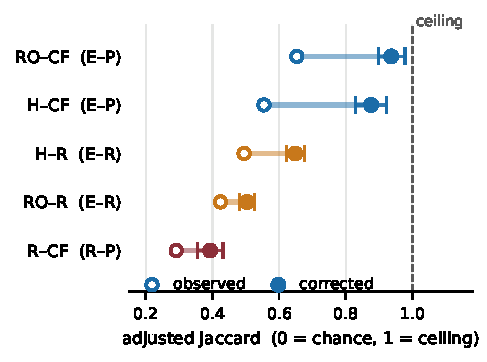
\includegraphics[width=\columnwidth]{F0_observed_vs_corrected.pdf}
\caption{Observed (hollow) vs.\ reliability-corrected (filled) agreement for the five cross-paradigm pairs, pooled; whiskers are bootstrap CIs on the corrected value. Correcting for instrument unreliability moves the two extraction--perturbation pairs to the ceiling but leaves every rationale-involving pair far short of it.}
\label{fig:dumbbell}
\end{figure}

Agreement is not flat across paradigm pairs (Table~\ref{tab:ladder}, Figure~\ref{fig:dumbbell}). Observed agreement follows a ladder ordered by paradigm distance---within-instance complete-case component means: E--P $0.615$ $>$ E--R $0.395$ $>$ R--P $0.286$ ($N{=}1{,}153$)---with the same-paradigm H--RO reference at $0.596$. Remarkably, the extraction--counterfactual pairs agree about as strongly as the two extraction methods agree with each other, \emph{before} any reliability correction.

The disattenuation resolves the ambiguity that a raw ladder leaves open. Correcting each pair by its instruments' self-consistency ceilings, the two extraction--perturbation pairs rise to $0.88$ and $0.94$---close to, though statistically just short of, the ceiling (both CIs exclude 1). In other words, \emph{most of the observed extraction$\leftrightarrow$counterfactual divergence is elicitation noise, not paradigm disagreement}: when a minimal edit exists and is found, it touches the same tokens the extractive paradigms score highest. By contrast, every rationale-involving pair stays far below its ceiling: H--R $0.649$, RO--R $0.504$, and R--CF $0.393$---even though the rationale is the \emph{most} reliable instrument ($\mathrm{rel}=0.89$), so its divergence cannot be blamed on noisy elicitation. The one-sentence free-text rationale systematically names different evidence than both the extractive and the counterfactual paradigms. A pre-registered soft-matching sensitivity (\S\ref{sec:robustness}) shows this is not lexical variation (synonyms explain ${\approx}0\%$ of the gap): rationales differ \emph{evidentially}.

Because a low reliability \emph{inflates} the corrected ratio, this reading depends on the ceilings being properties of the instruments rather than of one particular rewording. We therefore collected the ceilings under \emph{three} independent paraphrases of every elicitation prompt, across all 12 cells (\S\ref{sec:disatt}). Individual cells do move---Nova Pro's SST-2 CF reliability ranges $0.57$--$0.70$ across the three wordings---but pooled over cells the corrected values are stable: re-deriving Table~\ref{tab:ladder} under each paraphrase separately shifts every pair by at most $0.043$ (H--CF $0.853$--$0.895$; RO--CF $0.923$--$0.956$; R--CF $0.391$--$0.396$, a range of $0.005$), and the ordering never changes. Both extraction--perturbation pairs land just below the ceiling under all three. The remaining exposure is that the recovery simulation models \emph{independent} instrument noise, whereas the shared label anchor plausibly correlates errors across paradigms in the direction that inflates corrected values (Appendix~\ref{app:simulation}); and per-cell entries whose CF reliability nears the floor (e.g.\ DeepSeek-V3/AG News) still plausibly overshoot and carry at-ceiling flags for that reason. The rationale-divergence conclusion is exposed to none of this: R is the \emph{most} reliable instrument, the most paraphrase-stable one, and its corrected pairs sit $0.35$--$0.61$ below the ceiling.

The pattern is strongest exactly where shortcuts are broken: on CAD-IMDb, corrected R--CF falls to $0.12$--$0.36$ across models while five of the six corrected extraction--CF pairs lie between $0.90$ and $1.04$ (the exception is Nova Pro's H--CF at $0.53$; Appendix Table~\ref{tab:disattenuated}). This is consistent with the necessity/sufficiency distinction of \citet{mothilal2021towards}: attribution-style and counterfactual evidence coincide when one cue is both sufficient and necessary, but free-text rationalization drifts toward plausible narrative rather than the tokens that actually decide the flip.

\subsection{Explanations are paradigm-shaped, not model-shaped}
\label{sec:crossmodel}

\begin{table}[t]
\centering
\small
\setlength{\tabcolsep}{3.4pt}
\begin{tabular}{lccc}
\toprule
Dataset & Cross & Within & $\Delta_{\text{matched}}$ [95\% CI] \\
\midrule
SST-2    & 0.622 & 0.498 & $+0.129$ [0.073, 0.190] \\
MNLI     & 0.596 & 0.495 & $+0.046$ [0.009, 0.087] \\
AG News  & 0.569 & 0.491 & $+0.066$ [0.035, 0.100] \\
CAD-IMDb & 0.585 & 0.367 & $+0.218$ [0.187, 0.248] \\
\bottomrule
\end{tabular}
\caption{\textbf{Cross-model contrast} (AJ scale). Cross = same strategy, different models, mean AJ; Within = one model's cross-paradigm \ecsadj{}. $\Delta_{\text{matched}}$ is the pre-registered strategy-matched paired per-instance contrast ($\{$H, R, RO$\}$ cross-model pairs vs.\ the within-model extraction--rationalization component), which controls CF representation; all four CIs exclude 0.}
\label{tab:crossmodel}
\end{table}

If each explanation paradigm were a window onto a model-specific reasoning process, one model's four explanations should cohere more than two different models' renditions of the same paradigm. The opposite holds (Table~\ref{tab:crossmodel}): same-strategy agreement \emph{across} models exceeds cross-paradigm agreement \emph{within} a model on all four datasets, with the strategy-matched paired contrast positive everywhere (from $+0.046$ on MNLI to $+0.218$ on CAD-IMDb). The elicitation paradigm, not model identity, is the dominant factor shaping which evidence an explanation names. Practically: swapping the model changes the explanation less than swapping the question format.

Cross-model pairs are \emph{not} conditioned on the two models having predicted the same label: they agree on 93.9\% of the 8{,}074 pairs, and the remaining 6.1\% compare explanations of different predicted labels. This makes the contrast conservative---restricting to label-matched pairs could only raise the cross-model side---so the direction of the finding is unaffected.

\subsection{Consensus cores are causally load-bearing}
\label{sec:erasure}

\begin{table}[t]
\centering
\small
\setlength{\tabcolsep}{4.5pt}
\begin{tabular}{llcccc}
\toprule
Model & Op. & CC3 & Random & Gap & $p_{\mathrm{Holm}}$ \\
\midrule
DeepSeek-V3 & mask   & 0.316 & 0.123 & 0.192 & .0002 \\
DeepSeek-V3 & delete & 0.330 & 0.125 & 0.205 & .0002 \\
Nova Pro    & mask   & 0.291 & 0.147 & 0.144 & .0002 \\
Nova Pro    & delete & 0.311 & 0.132 & 0.179 & .0002 \\
Qwen3-235B  & mask   & 0.276 & 0.104 & 0.172 & .0002 \\
Qwen3-235B  & delete & 0.305 & 0.112 & 0.193 & .0002 \\
\bottomrule
\end{tabular}
\caption{\textbf{Family (b): consensus-core erasure.} Flip rate of the model's own prediction after erasing CC3 tokens (named by $\ge$3 strategies) vs.\ an occurrence-matched random content-word control; one-sided sign-flip permutation on within-instance paired differences, Holm across operators.}
\label{tab:erasure}
\end{table}

Do the tokens the paradigms agree on actually matter to the prediction? Erasing the CC3 consensus core flips the model's own prediction in $28$--$33\%$ of instances, versus $10$--$15\%$ for occurrence-matched random controls---a $2.0$--$2.7\times$ ratio, significant for every model under both erasure operators (Table~\ref{tab:erasure}; Figure~\ref{fig:erasure} in the appendix plots both panels). The gap grows monotonically with agreement tier (pooled, delete operator: $0.152 \to 0.206 \to 0.213$ for low/mid/high-\ecsadj{} terciles; descriptive). Following \citet{parcalabescu2024measuring}, we interpret this strictly as a second \emph{consistency} axis---stated evidence coincides with revealed input sensitivity---not as ground-truth faithfulness: the core is extracted from, and the flip verified by, the same model \citep{atanasova2020diagnostic,deyoung2020eraser}. The control is modest in what it rules out: matched-random shows consensus beats \emph{noise}, not that it beats any salient-token heuristic. The per-strategy arms of the same pass look at first like a challenge---whole evidence sets flip more often than the consensus core (H $0.44$--$0.45$, CF $0.45$--$0.49$ vs.\ CC3 $0.29$--$0.32$)---but those arms erase far more text: the mean H set holds $12.6$ tokens and CF $6.2$, against $3.1$ for CC3. Normalizing by tokens erased reverses the ordering. Per erased token, CC3 flips at $0.096$ (mask) and $0.103$ (delete), above every individual strategy---CF $0.072/0.079$, RO $0.072/0.078$, R $0.057/0.061$, H $0.035/0.036$---and roughly $2.5\times$ its size-matched random control ($0.041/0.040$). Consensus tokens are thus the \emph{densest} evidence per unit of text destroyed, which is the claim the erasure axis is meant to support. This normalization is a post-hoc descriptive comparison across arms of differing size, not a controlled test; the controlled version---a like-sized non-consensus salient baseline (single-strategy-only or top-TF-IDF tokens, matched to CC3's size)---is specified but not run here, and we flag it as the outstanding gap in this axis.

\subsection{Agreement does not predict simulatability under generic perturbations}
\label{sec:simulatability}

\begin{table*}[t]
\centering
\small
\begin{tabular}{lccccccc}
\toprule
& & \multicolumn{4}{c}{Simulatability gain over baseline} & & \\
\cmidrule(lr){3-6}
Target model & Baseline acc. & H & R & CF & RO & $\rho(\ecsadj,\text{gain})$ [95\% CI] & $p_{\mathrm{Holm}}$ \\
\midrule
Nova Pro    & 0.877 & $-0.009$ & $-0.002$ & $-0.006$ & $-0.001$ & $-0.011$ [$-0.155$, $0.144$] & 1.00 \\
Qwen3-235B  & 0.870 & $+0.005$ & $+0.012$ & $-0.069$ & $+0.003$ & $+0.006$ [$-0.141$, $0.172$] & 1.00 \\
DeepSeek-V3 & 0.767 & $+0.016$ & $+0.038$ & $+0.020$ & $+0.013$ & $-0.015$ [$-0.159$, $0.146$] & 1.00 \\
\midrule
Pooled      & 0.838 & $+0.004$ & $+0.016$ & $-0.015$ & $+0.005$ & $-0.001$ [$-0.091$, $0.088$] & --- \\
\bottomrule
\end{tabular}
\caption{\textbf{Family (c), pre-registered null.} Simulatability on 600 cohort instances under \emph{explanation-independent} perturbations (a deliberately strategy-fair variant of the explanation-derived construct of \citealp{chen2024models}; see text): a held-out simulator model predicts the target model's labels on perturbed inputs, given one strategy's explanation vs.\ no explanation. Explanations barely move simulator accuracy, and instance-level \ecsadj{} does not predict simulatability gain (c1 Spearman shown; the c2 tercile contrasts are likewise null, all Holm $p\ge0.99$).}
\label{tab:simulatability}
\end{table*}

Cross-paradigm agreement would be decision-relevant if it flagged when explanations fail their core job: helping an observer predict model behavior \citep{chen2024models}. One construct note: \citet{chen2024models} derive probe inputs from the explanation under evaluation, whereas our perturbations are deliberately explanation-\emph{independent} so that one perturbation set is fair to all four strategies. We therefore test whether explanations help predict behavior on \emph{generic} corruptions---a weaker claim than explanation-derived simulatability, and why we qualify this subsection's conclusions accordingly. The pre-registered test answers no (Table~\ref{tab:simulatability}). First, a stark descriptive fact: explanations barely help at all. Simulator accuracy with an explanation differs from the no-explanation baseline by $-0.07$ to $+0.04$; the largest gain (DeepSeek-V3 rationales, $+0.038$) is small, and counterfactuals \emph{hurt} simulation of Qwen3-235B ($-0.069$). Second, the registered association is null: instance-level \ecsadj{} does not correlate with simulatability gain for any model (c1: $|\rho|\le0.015$, all Holm $p{=}1.0$; c2 tercile contrasts: all Holm $p\ge0.99$), and a low-agreement ``red flag'' has precision $\le 0.04$ for identifying instances where explanations mislead. High baselines are part of the story (perturbed predictions are guessable from the text alone at $77$--$88\%$, leaving limited headroom), but the conclusion within this design is unambiguous: internal consistency among self-explanations is not a proxy for their utility to an observer \emph{on this task family}. Whether agreement predicts the stronger, explanation-derived simulatability construct remains open; testing it requires per-strategy perturbation sets and is the natural follow-up. We report this null as pre-registered; it constrains how our---and others'---agreement metrics should be used.

\subsection{Robustness}
\label{sec:robustness}

Six pre-registered sensitivity analyses (i--vi) and two post-hoc checks added in revision (vii--viii) probe the main results. \textbf{(i) Missingness:} complete-case membership is CF-gated (a verified minimal edit must exist). Substituting the unconstrained free-CF rewrite for the minimal one yields complete-case \ecsadj{} $0.382$ ($N{=}1{,}318$), positive in all cells: conclusions survive removing the minimal-edit gate. \textbf{(ii) Chance model:} the uniform null assumes evidence tokens are drawn uniformly from the instance vocabulary, whereas all strategies preferentially select salient-looking words; a frequency-weighted null shifts the pooled estimate by only $-0.011$ ($0.432\to0.421$), with every cell still positive. The shift is small by construction: the urn is the \emph{content-word} vocabulary after stopword removal and lemmatization, so the high-frequency function words that would otherwise dominate a frequency-weighted draw are already absent, leaving a comparatively flat weight distribution over the remaining candidates. \textbf{(iii) Lexical variation:} scoring with embedding-based soft matching (pinned static vectors, cosine $\tau{=}0.8$, matched MC null) leaves complete-case \ecsadj{} unchanged ($0.4320$ at $\tau{=}0.8$) and closes $\approx 0\%$ of the extraction--perturbation vs.\ rationale-pair gap ($+0.200$ hard vs.\ $+0.204$ soft): the rationale divergence of \S\ref{sec:ladder} is evidential, not synonymy. \textbf{(iv) Estimand family:} the available-component family (a2) reproduces 12/12 significance. \textbf{(v) Test conservativeness:} the AJ floor asymmetry makes the one-sided sign-flip test conservative by construction. \textbf{(vi) Confidence:} verbalized confidence is degenerate at temperature 0 (mean $0.94$ with heavy clustering at $0.95$), replicating \citet{xiong2024can}; its association with \ecsadj{} is weak and inconsistent (per-cell Spearman $-0.16$ to $+0.31$; Appendix Table~\ref{tab:confidence}) and we draw no conclusion from it. \textbf{(vii) Degeneracy exclusions} \emph{(post-hoc)}\textbf{:} the $\varepsilon$ guard drops pairs unevenly ($17.3\%$ of H--R and $17.0\%$ of H--CF slots vs.\ $2.5\%$ of RO--R), so we re-derived the ladder on the $850$ complete cases with \emph{no} degenerate pair: E--P $0.618 >$ E--R $0.451 >$ R--P $0.313$---same ordering as the full set ($0.615/0.395/0.286$), so the guard does not manufacture it (Appendix~\ref{app:degeneracy}). \textbf{(viii) Prediction correctness} \emph{(post-hoc)}\textbf{:} complete-case \ecsadj{} is $0.437$ on correct predictions ($n{=}1{,}085$) vs.\ $0.360$ on incorrect ones ($n{=}68$), with no consistent per-cell direction (Table~\ref{tab:correctness}): agreement is not an artifact of correct instances, though the incorrect stratum is too small for inference.

\section{Discussion}
\label{sec:discussion}

\paragraph{Paradigms are complements, not substitutes.} The reliability-corrected picture says the four standard ways of asking ``why'' collapse into roughly two evidential objects, not one and not four: an extraction/counterfactual cluster agreeing near its noise ceiling, and free-text rationalization, which reliably (in both senses) tells a different story. This cautions against averaging paradigms into one ``explanation quality'' score, and against treating a rationale as a cheap summary of token-level evidence---on shortcut-broken data the two are barely related (corrected R--P as low as $0.12$).

\paragraph{Measure the instrument before the construct.} Uncorrected, our data would ``show'' substantial extraction--counterfactual disagreement (observed $0.56$--$0.65$); about three quarters of that apparent shortfall is elicitation noise, which the paraphrase ceiling makes visible and the disattenuation removes. Agreement studies of LLM explanations should routinely report self-consistency ceilings---observed agreement without them conflates two very different failure modes.

\paragraph{Consistency $\neq$ utility.} The erasure result says consensus evidence is causally load-bearing; the simulatability null says none of this measurably helps an observer predict the model on generic corruptions of the input. Both can be true: our erasure perturbs the tokens explanations name, while simulatability requires explanations to transfer \emph{decision structure}, which one-shot label-conditioned explanations of high-accuracy classifiers apparently do not carry---at least under explanation-independent perturbations. Agreement metrics---ours included---should therefore be read as descriptions of the explanation-generating process, not as certificates of usefulness.

\section{Conclusion}
\label{sec:conclusion}

Four self-explanation paradigms, measured across three LLM families and four datasets under a pre-registered design, agree above chance everywhere---but not uniformly. Once instrument reliability is accounted for, counterfactual and extractive evidence coincide up to elicitation noise while free-text rationales diverge evidentially; the paradigm shapes the explanation more than the model does; consensus tokens are causally load-bearing; and none of this predicts simulatability under explanation-independent perturbations. The measurement stack (exact-null adjusted Jaccard, paradigm balancing, paraphrase ceilings, disattenuation) is model-agnostic and, we hope, useful wherever explanation agreement is quantified.

\section*{Limitations}
\label{sec:limitations}

\paragraph{Consistency, not faithfulness.} Every axis here---cross-paradigm agreement, erasure, simulatability---is a consistency measure among model outputs \citep{parcalabescu2024measuring,jacovi2020towards}. High agreement does not certify that any explanation reflects the model's computation; all four paradigms could converge on the same plausible-but-unfaithful cue.

\paragraph{Label-conditioned elicitation.} All explanation prompts reveal the model's predicted label, so we measure consistency of \emph{post-hoc rationalizations} \citep{wiegreffe2021measuring,turpin2023language}. The shared anchor could inflate agreement by pointing every strategy at the same obvious cue; the chance/ceiling adjustment does not remove this, and a no-label control is future work.

\paragraph{Counterfactual-driven selection.} Complete-case \ecsadj{} conditions on a verified minimal counterfactual existing; 1{,}153/2{,}400 instances (48\%) qualify. Complete and incomplete instances are indistinguishable on every agreement component measurable for both, on length, vocabulary, and accuracy, and the free-CF sensitivity reproduces all conclusions, but selection on unobservables cannot be excluded. Relatedly, the attribution$\leftrightarrow$intervention gap we quantify is partly definitional \citep{mothilal2021towards}: flip-sets and support-sets need not coincide; our contribution is measuring the size and reliability-adjusted reality of that gap, not adjudicating it as error.

\paragraph{Models and data.} Three mid-to-large model families---two open-weight, one proprietary---accessed through one provider; none is a current frontier system (an access constraint, not a design choice). All four datasets predate training cutoffs and are plausibly contaminated \citep{sainz2023nlp}; accuracy is 80--98\%, so we describe explanations of largely easy predictions---CAD-IMDb blunts the shortcut concern but not the contamination concern. English classification tasks only; generation and reasoning tasks are untested.

\paragraph{Instrument scope.} Reliability ceilings rest on three paraphrases per prompt over 50-instance cohorts. Three is enough to show that the pooled corrected values are not artifacts of one rewording (spread $\le 0.043$; \S\ref{sec:ladder}) but not enough to characterize the full distribution of paraphrases, and individual cells remain sensitive: a cell's reliability for one strategy moves by up to $0.26$ across wordings (DeepSeek-V3/MNLI, H), so per-cell corrected values should be read with wider uncertainty than their bootstrap CIs alone suggest. The ceilings are also paraphrase-stability estimates specifically, not full test--retest distributions --- they hold the model, decoding, and cohort fixed and vary only the wording. A distinct and unresolved exposure is that our validation of the correction (Appendix~\ref{app:simulation}) models instrument noise as \emph{independent} across strategies, whereas the shared predicted-label anchor plausibly correlates errors across paradigms. Correlated errors inflate observed agreement without inflating self-consistency, so they inflate the corrected ratio too---in the direction of the at-ceiling claim. That caveat does not touch the rationale-divergence result (\S\ref{sec:ladder}), which is a claim that corrected agreement is \emph{low}. Verbalized confidence is degenerate at temperature 0 and uninformative here. Simulatability used three perturbations per instance and one simulator per target; low power against very small effects cannot be excluded, though the point estimates are near-exactly zero.

\section*{Ethics Statement}
All data are public English-language benchmark texts; no human subjects, annotators, or personal data were involved. The study consumed approximately $7.1$M tokens of commercial LLM inference. Findings indicate that LLM self-explanations, while internally consistent above chance, are paradigm-dependent and of unproven utility to observers; deploying them as trust signals in high-stakes settings would be premature, and our results should not be cited as evidence that any studied model ``explains itself'' faithfully.

\section*{Reproducibility Statement}
The full pipeline (collection, parsing, normalization, metrics, statistics, figures), the frozen prompt templates with SHA-256 manifest, curated dataset files with datasheets, the dated pre-registration with all amendments, per-instance artifacts, and every number in this paper are generated from a single archived run (seed 42, temperature 0, checkpointed and resumable; $600{+}$ unit/property tests, including planted-agreement simulations validating the estimator and, added in revision, the disattenuation step). Analyses are labelled pre-registered or post-hoc at each point of use. Code and artifacts will be released upon publication.

% NOTE: the bib file is refs.bib, not references.bib — a sibling directory named
% `references/` (cited-paper PDFs) shadows the basename during BibTeX's file lookup,
% which fails as "Access is denied" when it opens the directory instead of the file.
\bibliography{refs}

\appendix

\section{Elicitation Prompts}
\label{app:prompts}

All strategies are elicited with frozen templates (SHA-256 manifest in the release); the classification and confidence prompts, and dataset-specific CF variants (multiclass label sets, NLI hypothesis editing), appear in the release. The four core templates, abridged to their instruction lines ($\{\cdot\}$ = filled fields; every prompt opens with \emph{``The text was classified as: \{predicted label\}''} and the text, and requests JSON-only output):

\begin{description}[leftmargin=1em,itemsep=2pt]
\item[H (highlighting).] ``Analyze the importance of each word for this classification. Give every word an importance score from 1 (irrelevant) to 10 (decisive), using each word exactly as it appears in the text, in order. Include every occurrence, even repeated words.''
\item[R (rationale).] ``In one sentence, explain why the text was classified as \{predicted label\}.''
\item[CF (counterfactual).] ``Edit the text so that it is classified as \{other label(s)\} instead. Make as few edits as possible---change at most a third of the words, and do not add new sentences. Keep the original spacing and punctuation style; only change the words you edit.''
\item[RO (rank ordering).] ``Identify the 5 most important words for this classification, ranked from most to least important. Each item must be a single word copied from the text.''
\end{description}

Each strategy also has a frozen semantically-equivalent paraphrase used only for the self-consistency ceiling (\S\ref{sec:disatt}).

\section{Coverage, Components, and Confidence}
\label{app:tables}

Table~\ref{tab:coverage} reports per-strategy validity and complete-case counts per cell. Table~\ref{tab:paradigms} reports the per-cell paradigm components (available-component means; the within-instance complete-case comparison is in \S\ref{sec:ladder}). Table~\ref{tab:confidence} reports the verbalized-confidence association, and Table~\ref{tab:correctness} the complete-case estimate split by prediction correctness. Figure~\ref{fig:heatmap} shows the component heatmap beside the raw-Jaccard view it replaces; Figure~\ref{fig:cftradeoff} shows the counterfactual validity--minimality trade-off; Figure~\ref{fig:confgrid} the confidence--agreement grid.

\begin{table*}[t]
\centering
\small
\caption{Per-strategy extraction success and complete-case counts, per model$\times$dataset.}
\label{tab:coverage}
\begin{tabular}{lrrrrrr}
\toprule
Cell & N & H & R & CF & RO & Complete \\
\midrule
DeepSeek-V3/AG News & 200 & 1.000 & 0.960 & 0.415 & 1.000 & 81 \\
DeepSeek-V3/CAD-IMDb & 200 & 1.000 & 1.000 & 0.985 & 1.000 & 197 \\
DeepSeek-V3/MNLI & 200 & 1.000 & 0.965 & 0.460 & 0.965 & 88 \\
DeepSeek-V3/SST-2 & 200 & 1.000 & 0.955 & 0.905 & 0.990 & 172 \\
Nova Pro/AG News & 200 & 0.995 & 0.950 & 0.155 & 1.000 & 31 \\
Nova Pro/CAD-IMDb & 200 & 0.965 & 0.985 & 0.920 & 0.995 & 177 \\
Nova Pro/MNLI & 200 & 0.995 & 0.940 & 0.355 & 0.970 & 65 \\
Nova Pro/SST-2 & 200 & 0.990 & 0.960 & 0.650 & 0.990 & 124 \\
Qwen3-235B/AG News & 200 & 0.975 & 0.975 & 0.075 & 1.000 & 15 \\
Qwen3-235B/CAD-IMDb & 200 & 0.955 & 0.990 & 0.930 & 1.000 & 179 \\
Qwen3-235B/MNLI & 200 & 0.945 & 0.990 & 0.400 & 0.975 & 77 \\
Qwen3-235B/SST-2 & 200 & 1.000 & 0.940 & 0.810 & 0.985 & 149 \\
\bottomrule
\end{tabular}
\end{table*}

\begin{table}[t]
\centering
\small
\caption{Paradigm-component adjusted Jaccard: E--R, E--P, R--P per cell.}
\label{tab:paradigms}
\begin{tabular}{lrrr}
\toprule
Cell & E--R & E--P & R--P \\
\midrule
DeepSeek-V3/AG News & 0.556 & 0.522 & 0.456 \\
DeepSeek-V3/CAD-IMDb & 0.403 & 0.704 & 0.277 \\
DeepSeek-V3/MNLI & 0.526 & 0.501 & 0.367 \\
DeepSeek-V3/SST-2 & 0.522 & 0.770 & 0.581 \\
Nova Pro/AG News & 0.446 & 0.376 & 0.275 \\
Nova Pro/CAD-IMDb & 0.233 & 0.531 & 0.090 \\
Nova Pro/MNLI & 0.531 & 0.248 & 0.191 \\
Nova Pro/SST-2 & 0.442 & 0.485 & 0.331 \\
Qwen3-235B/AG News & 0.490 & 0.444 & 0.410 \\
Qwen3-235B/CAD-IMDb & 0.251 & 0.703 & 0.138 \\
Qwen3-235B/MNLI & 0.543 & 0.477 & 0.338 \\
Qwen3-235B/SST-2 & 0.339 & 0.750 & 0.258 \\
\bottomrule
\end{tabular}
\end{table}

\begin{table}[t]
\centering
\small
\setlength{\tabcolsep}{3.5pt}
\caption{Confidence$\leftrightarrow$ECS association (Spearman $\rho$, Kendall $\tau_b$), per cell.}
\label{tab:confidence}
\begin{tabular}{lrrrr}
\toprule
Cell & $\rho$ & $\tau_b$ & $p$ & N \\
\midrule
DeepSeek-V3/AG News & -0.113 & -0.090 & 0.1177 & 194 \\
DeepSeek-V3/CAD-IMDb & 0.310 & 0.235 & 0.0000 & 200 \\
DeepSeek-V3/MNLI & 0.026 & 0.020 & 0.7172 & 192 \\
DeepSeek-V3/SST-2 & 0.215 & 0.169 & 0.0024 & 198 \\
Nova Pro/AG News & -0.164 & -0.130 & 0.0244 & 189 \\
Nova Pro/CAD-IMDb & 0.079 & 0.062 & 0.2702 & 197 \\
Nova Pro/MNLI & 0.207 & 0.156 & 0.0046 & 187 \\
Nova Pro/SST-2 & 0.209 & 0.164 & 0.0034 & 194 \\
Qwen3-235B/AG News & -0.009 & -0.005 & 0.9065 & 190 \\
Qwen3-235B/CAD-IMDb & 0.146 & 0.112 & 0.0410 & 196 \\
Qwen3-235B/MNLI & 0.122 & 0.092 & 0.0973 & 186 \\
Qwen3-235B/SST-2 & 0.175 & 0.137 & 0.0137 & 198 \\
\bottomrule
\end{tabular}
\end{table}

% Generated by paper/tables/make_correctness_table.py from the run of record.
\begin{table}[t]
\centering
\small
\setlength{\tabcolsep}{4pt}
\begin{tabular}{lrrrr}
\toprule
 & \multicolumn{2}{c}{Correct} & \multicolumn{2}{c}{Incorrect} \\
\cmidrule(lr){2-3}\cmidrule(lr){4-5}
Cell & \ecsadj & $N$ & \ecsadj & $N$ \\
\midrule
DeepSeek-V3/AG News & 0.505 & 70 & 0.483 & 10 \\
DeepSeek-V3/CAD-IMDb & 0.475 & 187 & 0.154 & 6 \\
DeepSeek-V3/MNLI & 0.463 & 40 & 0.360 & 11 \\
DeepSeek-V3/SST-2 & 0.615 & 140 & 0.705 & 3 \\
Nova Pro/AG News & 0.350 & 27 & 0.398 & 3 \\
Nova Pro/CAD-IMDb & 0.306 & 145 & 0.222 & 9 \\
Nova Pro/MNLI & 0.297 & 33 & 0.171 & 4 \\
Nova Pro/SST-2 & 0.406 & 102 & 0.530 & 7 \\
Qwen3-235B/AG News & 0.427 & 14 & --- & 0 \\
Qwen3-235B/CAD-IMDb & 0.372 & 170 & 0.345 & 8 \\
Qwen3-235B/MNLI & 0.469 & 35 & 0.095 & 4 \\
Qwen3-235B/SST-2 & 0.444 & 122 & 0.646 & 3 \\
\midrule
Pooled & 0.437 & 1085 & 0.360 & 68 \\
\bottomrule
\end{tabular}
\caption{Complete-case \ecsadj{} split by whether the model's prediction was correct. Descriptive only: the incorrect stratum is small (68 of 1{,}153 complete cases) and the per-cell direction is inconsistent (agreement is higher on incorrect predictions in 4 of 11 estimable cells).}
\label{tab:correctness}
\end{table}


\section{Validating the Disattenuation on the AJ Scale}
\label{app:simulation}

Spearman's correction is derived for product-moment correlations; we apply it to mean adjusted-Jaccard agreement, so we validate the analogue by simulation rather than assume it.

\paragraph{Design.} Each instrument observes a latent evidence set $T_s \subseteq V$. One elicitation keeps each token of $T_s$ independently with probability $q_s$ and replaces each dropped token with a uniform random distractor---size-preserving, matching AJ's fixed-size geometry. For a configuration $(V,a,b,\text{overlap},q_A,q_B)$ we draw 2{,}000 elicitation pairs and compute $\mathrm{rel}_s$ as mean $\aj$ between two independent elicitations of the same $T_s$, $\mathrm{obs}$ as mean $\aj$ across instruments, and $\mathrm{true}=\aj(T_A,T_B)$ noise-free. The grid crosses four geometries (balanced, imbalanced, large-$V$, small-$V$), $q\in\{0.55,0.7,0.85,1.0\}$, and three planted overlap levels: 120 configurations, 66 above the pre-registered floor.

\paragraph{Result.} Above the floor, disattenuation recovers the planted value with mean $|\mathrm{corrected}-\mathrm{true}|=0.050$, against mean $|\mathrm{obs}-\mathrm{true}|=0.260$ on the noisy configurations---a fourfold error reduction. Bias depends on reliability: in the band $\min(\mathrm{rel})\ge0.60$ recovery is essentially unbiased (signed bias $+0.009$, max error $0.041$), in $[0.45,0.60)$ bias is $+0.047$, and in $[0.30,0.45)$ it reaches $+0.072$ (max $+0.156$, on configurations with planted agreement $1.0$). Below the floor, maximum error grows to $0.245$. Two consequences for the paper: every pooled pair in Table~\ref{tab:ladder} sits in the unbiased regime (lowest pooled reliability is CF at $0.62$), and the upward near-floor bias means low-reliability \emph{per-cell} entries should be read as upper bounds---which is what the at-ceiling flag marks. These assertions are pinned in the released test suite, in \texttt{tests/} as \texttt{test\_disattenuation\_\allowbreak recovery.py}.

\paragraph{Scope.} The simulation draws each instrument's noise independently. It therefore validates the correction's algebra on the AJ scale but does \emph{not} cover correlated instrument errors, which our design plausibly induces: every strategy is conditioned on the same predicted label (\S Limitations), so the paradigms may err toward the same salient token together. Correlated errors raise observed agreement without raising same-strategy self-consistency, and so inflate the corrected ratio. The at-ceiling reading is the claim exposed to this; the rationale-divergence reading, being a claim of \emph{low} corrected agreement, is if anything conservative under it.

\section{Paraphrase Spread of the Reliability Ceilings}
\label{app:paraphrase}

Each of the four elicitation prompts has three independent rewordings (the originally registered paraphrase plus two added in revision). All preserve the format slots and the JSON response schema; only surface wording differs. Every ceiling in Table~\ref{tab:ladder} pools all three.

\paragraph{Ceilings move with wording; pooled corrected values do not.} Per cell the choice of rewording matters: Nova Pro's SST-2 ceilings span $0.50$--$0.59$ (H), $0.57$--$0.70$ (CF) and $0.70$--$0.81$ (RO) across the three, and the rationale instrument is the most stable ($0.86$--$0.90$). Pooled across the twelve cells, however, that variation largely averages out. Re-deriving the whole overall table under each rewording \emph{separately} gives:

\begin{center}
\small
\setlength{\tabcolsep}{4pt}
\begin{tabular}{lcccc}
\toprule
Pair & wording 1 & wording 2 & wording 3 & range \\
\midrule
RO--CF & 0.956 & 0.923 & 0.931 & 0.034 \\
H--CF  & 0.883 & 0.895 & 0.853 & 0.043 \\
H--R   & 0.654 & 0.666 & 0.628 & 0.038 \\
RO--R  & 0.516 & 0.499 & 0.499 & 0.017 \\
R--CF  & 0.391 & 0.396 & 0.392 & 0.005 \\
\bottomrule
\end{tabular}
\end{center}

No pair moves by more than $0.043$, the ordering is identical under all three wordings, and the rationale--perturbation contrast is the most stable quantity in the study ($0.005$). The single-paraphrase design would have reported RO--CF as $0.956$ with a CI that includes 1; pooling three rewordings gives $0.936$ with a CI that excludes it, which is why we describe the extraction--perturbation pairs as approaching rather than reaching the ceiling.

\section{Degeneracy Exclusions by Pair Type}
\label{app:degeneracy}

The $\varepsilon=0.10$ guard removes pairs whose geometry puts the ceiling within $\varepsilon$ of the chance floor, i.e.\ $J_{\max}-\mathbb{E}[J]<\varepsilon$. Exclusion rates differ sharply by pair type: H--R $17.3\%$ of elicited slots ($396/2286$), H--CF $17.0\%$ ($238/1397$), R--CF $13.7\%$ ($189/1375$), RO--CF $4.8\%$ ($67/1403$), RO--R $2.5\%$ ($58/2304$); RO's fixed 5-token sets rarely produce degenerate geometry.

\paragraph{Two distinct regimes.} The condition can be met from either side, and which one fires is dataset-dependent:

\begin{description}[leftmargin=1em,itemsep=1pt,topsep=2pt]
\item[(a) Small vocabulary.] On short inputs $V$ is small, so $\mathbb{E}[J]$ is large and rises to meet an otherwise healthy ceiling. This is a genuinely short-input effect: it accounts for $65$ of SST-2's exclusions (median $V=10$) and $41$ of MNLI's (median $V=12$), where the degenerate pairs average $\mathbb{E}[J]=0.37$ and $0.18$ respectively.
\item[(b) Extreme size imbalance.] $J_{\max}=\min/\max$ is itself below $\varepsilon$ regardless of $V$, because one evidence set is far larger than the other. Here chance is negligible---degenerate pairs average $\mathbb{E}[J]\approx0.045$---and the ceiling alone is the binding constraint.
\end{description}

Regime (b) is the dominant one and, importantly, is \emph{not} confined to short inputs. CAD-IMDb---our \emph{longest} inputs, paragraph-length reviews with median $V=68$---tops the exclusion counts at $398$ pair-slots, and every one of them is regime (b): its median H set holds $30$ tokens against a median CF set of $11$ and R of $6$, giving a median $J_{\max}$ of $0.108$ among excluded pairs. AG News is likewise $48/48$ regime (b). MNLI ($248$ of $289$) and SST-2 ($148$ of $213$) mix the two, since short premises produce both small $V$ and one-token counterfactuals. Totals: CAD-IMDb $398$, MNLI $289$, SST-2 $213$, AG News $48$ ($948$, reconciling with the pair-type view above).

Because the guard falls hardest on H- and CF-involving pairs, it could in principle shape the ladder. It does not: restricting to the $850$ complete cases containing \emph{no} degenerate pair reproduces the ordering and the separations (E--P $0.618$, E--R $0.451$, R--P $0.313$; full complete-case set $0.615$, $0.395$, $0.286$). E--R rises the most under the restriction ($+0.056$), which narrows the E--P/E--R gap while leaving R--P clearly lowest.

\section{Disattenuated Agreement, Per Cell}
\label{app:disatt}

Table~\ref{tab:disattenuated} reports, for every cell and pair: observed AJ, the two reliabilities, the corrected value with bootstrap CI, at-ceiling flags, and the pre-registered floor exclusions (CF on Nova Pro/AG News, where CF paraphrase reliability is $0.10$).

\begin{table*}[t]
\centering
\footnotesize
\caption{Disattenuated cross-paradigm agreement (Spearman 1904): observed AJ corrected by the geometric mean of the two strategies' self-consistency ceilings, per cell. Pairs below the pre-registered reliability floor (0.30, ceiling $n \geq 10$) are reported as excluded.}
\label{tab:disattenuated}
\begin{tabular}{llrrrl}
\toprule
Cell & Pair & Obs. & $rel_A{\times}rel_B$ & Corrected [95\% CI] & Flag \\
\midrule
DeepSeek-V3/AG News & H--R & 0.534 & 0.730$\times$0.910 & 0.655 [0.571, 0.738] &  \\
DeepSeek-V3/AG News & RO--R & 0.548 & 0.727$\times$0.910 & 0.674 [0.599, 0.757] &  \\
DeepSeek-V3/AG News & H--CF & 0.569 & 0.730$\times$0.316 & 1.185 [0.940, 1.569] & at ceiling \\
DeepSeek-V3/AG News & RO--CF & 0.479 & 0.727$\times$0.316 & 1.000 [0.776, 1.343] & at ceiling \\
DeepSeek-V3/AG News & R--CF & 0.456 & 0.910$\times$0.316 & 0.851 [0.638, 1.178] &  \\
DeepSeek-V3/CAD-IMDb & H--R & 0.631 & 0.603$\times$0.762 & 0.931 [0.830, 1.045] &  \\
DeepSeek-V3/CAD-IMDb & RO--R & 0.345 & 0.847$\times$0.762 & 0.430 [0.372, 0.495] &  \\
DeepSeek-V3/CAD-IMDb & H--CF & 0.616 & 0.603$\times$0.809 & 0.881 [0.804, 0.962] &  \\
DeepSeek-V3/CAD-IMDb & RO--CF & 0.797 & 0.847$\times$0.809 & 0.962 [0.901, 1.032] &  \\
DeepSeek-V3/CAD-IMDb & R--CF & 0.277 & 0.762$\times$0.809 & 0.353 [0.300, 0.406] &  \\
DeepSeek-V3/MNLI & H--R & 0.495 & 0.615$\times$0.950 & 0.647 [0.543, 0.760] &  \\
DeepSeek-V3/MNLI & RO--R & 0.551 & 0.750$\times$0.950 & 0.653 [0.568, 0.751] &  \\
DeepSeek-V3/MNLI & H--CF & 0.338 & 0.615$\times$0.648 & 0.535 [0.163, 0.915] &  \\
DeepSeek-V3/MNLI & RO--CF & 0.546 & 0.750$\times$0.648 & 0.783 [0.569, 1.021] &  \\
DeepSeek-V3/MNLI & R--CF & 0.367 & 0.950$\times$0.648 & 0.468 [0.248, 0.721] &  \\
DeepSeek-V3/SST-2 & H--R & 0.498 & 0.728$\times$0.957 & 0.596 [0.498, 0.708] &  \\
DeepSeek-V3/SST-2 & RO--R & 0.547 & 0.829$\times$0.957 & 0.614 [0.521, 0.711] &  \\
DeepSeek-V3/SST-2 & H--CF & 0.753 & 0.728$\times$0.679 & 1.071 [0.927, 1.244] & at ceiling \\
DeepSeek-V3/SST-2 & RO--CF & 0.778 & 0.829$\times$0.679 & 1.037 [0.913, 1.196] & at ceiling \\
DeepSeek-V3/SST-2 & R--CF & 0.581 & 0.957$\times$0.679 & 0.721 [0.596, 0.854] &  \\
Nova Pro/AG News & H--R & 0.443 & 0.547$\times$0.922 & 0.624 [0.535, 0.718] &  \\
Nova Pro/AG News & RO--R & 0.450 & 0.621$\times$0.922 & 0.594 [0.511, 0.682] &  \\
Nova Pro/AG News & H--CF & 0.379 & 0.547$\times$0.164 & -- & excl.: rel.\ floor (CF) \\
Nova Pro/AG News & RO--CF & 0.332 & 0.621$\times$0.164 & -- & excl.: rel.\ floor (CF) \\
Nova Pro/AG News & R--CF & 0.275 & 0.922$\times$0.164 & -- & excl.: rel.\ floor (CF) \\
Nova Pro/CAD-IMDb & H--R & 0.444 & 0.464$\times$0.804 & 0.728 [0.611, 0.856] &  \\
Nova Pro/CAD-IMDb & RO--R & 0.201 & 0.680$\times$0.804 & 0.272 [0.217, 0.334] &  \\
Nova Pro/CAD-IMDb & H--CF & 0.318 & 0.464$\times$0.717 & 0.552 [0.476, 0.640] &  \\
Nova Pro/CAD-IMDb & RO--CF & 0.740 & 0.680$\times$0.717 & 1.060 [0.967, 1.173] & at ceiling \\
Nova Pro/CAD-IMDb & R--CF & 0.090 & 0.804$\times$0.717 & 0.119 [0.065, 0.174] &  \\
Nova Pro/MNLI & H--R & 0.529 & 0.664$\times$0.922 & 0.676 [0.572, 0.787] &  \\
Nova Pro/MNLI & RO--R & 0.536 & 0.775$\times$0.922 & 0.635 [0.548, 0.729] &  \\
Nova Pro/MNLI & H--CF & 0.330 & 0.664$\times$0.346 & 0.690 [0.230, 1.217] &  \\
Nova Pro/MNLI & RO--CF & 0.171 & 0.775$\times$0.346 & 0.331 [0.007, 0.723] &  \\
Nova Pro/MNLI & R--CF & 0.191 & 0.922$\times$0.346 & 0.338 [-0.028, 0.756] &  \\
Nova Pro/SST-2 & H--R & 0.466 & 0.533$\times$0.903 & 0.672 [0.551, 0.813] &  \\
Nova Pro/SST-2 & RO--R & 0.415 & 0.698$\times$0.903 & 0.522 [0.407, 0.655] &  \\
Nova Pro/SST-2 & H--CF & 0.431 & 0.533$\times$0.698 & 0.706 [0.541, 0.882] &  \\
Nova Pro/SST-2 & RO--CF & 0.541 & 0.698$\times$0.698 & 0.775 [0.637, 0.931] &  \\
Nova Pro/SST-2 & R--CF & 0.331 & 0.903$\times$0.698 & 0.417 [0.271, 0.558] &  \\
Qwen3-235B/AG News & H--R & 0.487 & 0.700$\times$0.943 & 0.600 [0.526, 0.678] &  \\
Qwen3-235B/AG News & RO--R & 0.480 & 0.804$\times$0.943 & 0.552 [0.492, 0.618] &  \\
Qwen3-235B/AG News & H--CF & 0.465 & 0.700$\times$0.736 & 0.649 [0.324, 1.034] &  \\
Qwen3-235B/AG News & RO--CF & 0.434 & 0.804$\times$0.736 & 0.565 [0.272, 0.909] &  \\
Qwen3-235B/AG News & R--CF & 0.410 & 0.943$\times$0.736 & 0.492 [0.169, 0.867] &  \\
Qwen3-235B/CAD-IMDb & H--R & 0.622 & 0.600$\times$0.902 & 0.846 [0.746, 0.944] &  \\
Qwen3-235B/CAD-IMDb & RO--R & 0.163 & 0.816$\times$0.902 & 0.189 [0.145, 0.236] &  \\
Qwen3-235B/CAD-IMDb & H--CF & 0.647 & 0.600$\times$0.797 & 0.935 [0.858, 1.018] &  \\
Qwen3-235B/CAD-IMDb & RO--CF & 0.752 & 0.816$\times$0.797 & 0.932 [0.864, 1.014] &  \\
Qwen3-235B/CAD-IMDb & R--CF & 0.138 & 0.902$\times$0.797 & 0.163 [0.117, 0.212] &  \\
Qwen3-235B/MNLI & H--R & 0.549 & 0.735$\times$0.963 & 0.653 [0.565, 0.745] &  \\
Qwen3-235B/MNLI & RO--R & 0.533 & 0.729$\times$0.963 & 0.637 [0.543, 0.738] &  \\
Qwen3-235B/MNLI & H--CF & 0.506 & 0.735$\times$0.630 & 0.744 [0.424, 1.081] &  \\
Qwen3-235B/MNLI & RO--CF & 0.427 & 0.729$\times$0.630 & 0.630 [0.386, 0.886] &  \\
Qwen3-235B/MNLI & R--CF & 0.338 & 0.963$\times$0.630 & 0.435 [0.151, 0.720] &  \\
Qwen3-235B/SST-2 & H--R & 0.319 & 0.720$\times$0.849 & 0.408 [0.293, 0.530] &  \\
Qwen3-235B/SST-2 & RO--R & 0.359 & 0.762$\times$0.849 & 0.446 [0.333, 0.565] &  \\
Qwen3-235B/SST-2 & H--CF & 0.744 & 0.720$\times$0.790 & 0.987 [0.861, 1.133] &  \\
Qwen3-235B/SST-2 & RO--CF & 0.751 & 0.762$\times$0.790 & 0.967 [0.856, 1.096] &  \\
Qwen3-235B/SST-2 & R--CF & 0.258 & 0.849$\times$0.790 & 0.315 [0.186, 0.443] &  \\
\bottomrule
\end{tabular}
\end{table*}


\begin{figure*}[t]
\centering

\includegraphics[width=\textwidth]{F2_ecs_adj_distributions.pdf}
\caption{Per-instance \ecsadj{} distributions by model (rows) and dataset (columns); dashed line = cell mean; dark points = complete-case instances. All 12 cell means are above chance (Table~\ref{tab:primary}), but distributions are wide and often bimodal.}
\label{fig:distributions}
\end{figure*}

\begin{figure*}[t]
\centering

\includegraphics[width=0.98\textwidth]{F4_erasure_gap.pdf}
\caption{Consensus-core erasure. (a) CC3-minus-random flip-rate gap per model and operator (all Holm $p<.05$). (b) Pooled gap by \ecsadj{}-lift tier (descriptive): higher cross-paradigm agreement coincides with a larger causal-sensitivity gap.}
\label{fig:erasure}
\end{figure*}

\begin{figure*}[t]
\centering

\includegraphics[width=\textwidth]{F1_pairwise_heatmap.pdf}
\caption{(a) \ecsadj{} paradigm components per cell (primary scale). (b) The raw pairwise Jaccard view of the same data (deprecated comparator): without chance/ceiling adjustment, set-size geometry dominates the picture.}
\label{fig:heatmap}
\end{figure*}

\begin{figure}[t]
\centering

\includegraphics[width=\columnwidth]{F5_cf_tradeoff.pdf}
\caption{Counterfactual validity--minimality trade-off: minimal-edit CFs flip less often but edit far less; free rewrites flip reliably (90\%) but over-edit.}
\label{fig:cftradeoff}
\end{figure}

\begin{figure}[t]
\centering

\includegraphics[width=\columnwidth]{F7_confidence_ecs_grid.pdf}
\caption{Verbalized confidence vs.\ \ecsadj{} per cell. Confidence is degenerate at temperature 0 (clustered at 0.95), consistent with \citet{xiong2024can}; associations are weak and inconsistent.}
\label{fig:confgrid}
\end{figure}

\end{document}
